\subsection{Geometric Impedance}
\label{sec:imp_geo_imp}

Geometric impedances are characterised by resonant fields at a resonant frequency, typically characterised by some characteristic dimension of the structure. This is typically a characteristic length of a structure (cavity size, antenna length), which may be part of a vacuum tank, or an internal structure to the device exhibiting the resonance. 

As a simple example, consider a cylindrical pillbox cavity of radius $r_{cav}$ and length $L$ connected to a beam pipe of radius $r_{pipe}$ located at the centre of the cavity, as shown in Fig.~\ref{fig:cylin_geo_diagram}. For simplicity we shall assume that the cavity is made from a perfectly conducting materials. It shall be assumed that the fields do not propogate along the attached beam pipe (i.e. for frequencies below cutoff). In this example we shall consider a particle travelling on the axis of the beam pipe, and only the longitudinal wakefunction/impedance will be investigated to simplify matters. Further details can be found in [cite Andy Wolzski, E Jensen, Stupakov]. It can be shown that there are two families of resonant modes in in a pillbox cavity, TM-type modes and TE-type modes. The TE-type modes have no longitudinal electrical field by definition, and therefore do not contribute to the longitudinal wakefunction for an on axis particle. In a cylindrical coordinate system using coordinates $(r, \theta, z)$, the longitudinal electrical field of the $n$-th order TM-type modes can be shown to be

\begin{equation}
E_{z,n} = E_{0}J_{n}\left( k_{r} r \right) cos \left( n \theta \right) cos \left( k_{z} z \right) e^{-j \omega t}
\end{equation}

where $E_{0}$ is the magnitude of the electric field, $J_{n}$ is $n$-th order Bessel function, $k_{z}=n\pi{}/L$, and n is an interger. A wakefunction for each mode subsequently be defined as $w_{\parallel ,n}\left( \tau \right)$, where the total wakefunction is thus defined as

\begin{equation}
w_{\parallel} \left( \mathbf{r}_{1}, \mathbf{r}_{2}, \tau \right) =  \displaystyle\sum\limits_{n = 0}^{\infty} w_{\parallel ,n} \left( \tau \right) = \displaystyle\sum\limits_{n = 0}^{\infty} \int^{\infty}_{-\infty} dz E_{z,n} \left( r, \theta , z \right)
\end{equation}

\begin{figure}
\begin{center}
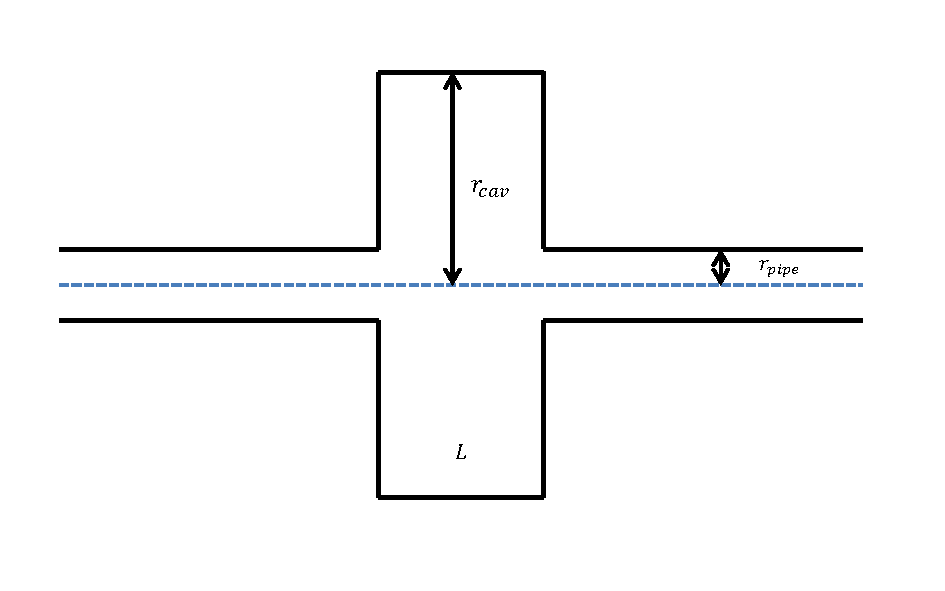
\includegraphics[width=0.7\textwidth]{Wakefields_and_Impedances/figures/pillbox-cav.pdf}
\end{center}
\caption{Cross section of a cylindrical pillbox cavity with an attached beam pipe}
\label{fig:cylin_geo_diagram}
\end{figure}

To evaluate the problem in the frequency domain we shall introduce the RLC parallel circuit model to simplif the frequency doman representation.

\subsubsection{RLC Circuit Model}

We can define any given resonance by an equivalent RLC circuit, which is driven by a current, shown in Fig.~\ref{fig:rlc_circ}. The symbols represent the equivalent resistor (R), inductance (L) and capcitance (C). From this circuit a number of defining parameters are now deduced, and the physical equivalents in the physical cavity are described.

\begin{figure}
\begin{center}
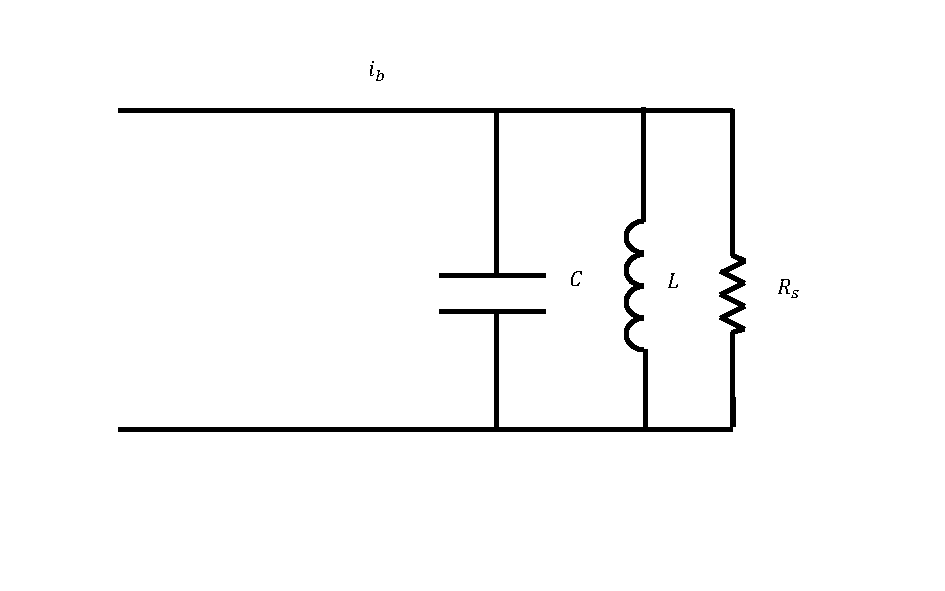
\includegraphics[width=0.7\textwidth]{Wakefields_and_Impedances/figures/equiv-circuit.pdf}
\end{center}
\caption{The equivalent RLC parallel circuit for a cavity resonance, driven by a current $i_{b}$, in this cas the beam current}
\label{fig:rlc_circ}
\end{figure}

The first parameter to be derived is the resonant frequency of the cavity mode itself $\omega_{0}$. This can be shown (by solving the time varying voltage build up of the circuit in Fig.~\ref{fig:rlc_circ}) to be given by

\begin{equation}
\omega_{0} = \frac{1}{LC}.
\end{equation}

Next we define the quality factor of the cavity mode, $Q_{n}$. This factor describes the damping of the wakefunction in the cavity for a given mode, larger values indicating a longer damping time. In terms of the cavity it is given by

\begin{equation}
Q_{n} = \frac{\omega_{0} W}{P_{loss}} = \omega_{0}RC
\end{equation}

where $W = \int_{V} \epsilon / 2 \left| \mathbf{E} \right|^{2} dV$ is the stored electromagnetic energy in the cavity due to the mode, and $P_{loss}$ is the total losses in the cavity. Commonly the later is dominated by conductive losses on the cavity walls, but as will be seen in later sections, also includes losses due to other mechanisms. The final figures of merit are the $R_{s, n}/Q_{n}$ of the cavity mode, and the shunt impedance $R_{s, n}$ of the mode. $R_{s, n}/Q_{n}$ is given by

\begin{equation}
\frac{R_{s, n}}{Q_{n}} = \frac{\left| V_{acc} \right|^{2}}{2 \omega_{0} W}
\end{equation}

where $V_{acc} = \int^{\infty}_{-\infty} E_{z, n} e^{-j \omega_{0} z/ \beta{}c} dz$ is the effective voltage that a traversing particle sees due to the cavity mode. It can thus be seen that the $R_{s, n}/Q_{n}$ of a cavity mode gives some ratio of the acceleration of a traversing particle to the stored energy. The shunt impedance $R_{s, n}$ is then given by

\begin{equation}
R_{s, n} = \left(  \frac{R_{s, n}}{Q){n}} \right) Q_{n} = \frac{\left| V_{acc} \right|^{2}}{2 P_{loss}}
\end{equation}

or an equivalent ratio for power loss in the cavity to acceleration of the particle. From these quality factors is defined a broadband description of the beam coupling impedance at all frequencies due to all modes, given by

\begin{equation}
Z_{\parallel} \left( \omega \right) = \displaystyle\sum\limits_{n = 0}^{\infty} Z_{\parallel, n} \left( \omega \right) = \displaystyle\sum\limits_{n = 0}^{\infty} \frac{R_{s, n}}{1 - iQ \left( \frac{\omega}{\omega_{0}} - \frac{\omega_{0}}{\omega} \right)}.
\end{equation}

And number of examples of this type of impedance are shown in Sec.~\ref{sec:beam_induced_heating}